% -*- coding: utf-8 -*-
%\nonstopmode
\documentclass[a4paper,10pt]{article}
\usepackage[polish]{babel}
\usepackage{polski}
%\usepackage[utf8]{inputenc}
\usepackage[T1]{fontenc}
\usepackage{marvosym}
\usepackage{fontspec} 					%for loading fonts
\usepackage{xunicode,xltxtra,url,parskip} 	%other packages for formatting
\RequirePackage{color,graphicx}
\usepackage[usenames,dvipsnames]{xcolor}
\usepackage[big]{layaureo} 				%better formatting of the A4 page
% an alternative to Layaureo can be ** \usepackage{fullpage} **
\usepackage{supertabular} 				%for Grades
\usepackage{titlesec}					%custom \section

%Setup hyperref package, and colours for links
\usepackage{hyperref}
\usepackage{enumerate}
\definecolor{linkcolour}{rgb}{0,0.2,0.6}
\hypersetup{colorlinks,breaklinks,urlcolor=linkcolour, linkcolor=linkcolour}

%FONTS
\defaultfontfeatures{Mapping=tex-text}
%\setmainfont[SmallCapsFont = Fontin SmallCaps]{Fontin}

\titleformat{\section}{\Large\scshape\raggedright}{}{0em}{}[\titlerule]
\titlespacing{\section}{0pt}{3pt}{3pt}
%Tweak a bit the top margin
\addtolength{\voffset}{-1.3cm}

%Italian hyphenation for the word: ''corporations''
\hyphenation{im-pre-se}

%-------------WATERMARK TEST [**not part of a CV**]---------------
\usepackage{textpos}

\setlength{\TPHorizModule}{10pt} %controls horizontal movements
\setlength{\TPVertModule}{10pt}  %controls vertical movements

%%%%%%%%%%%%%%%%%%%%%%%%%%%%%%%%%%%%%%%%%%%%%%%%%%%%%%%%%%
%--------------------BEGIN DOCUMENT----------------------%
%%%%%%%%%%%%%%%%%%%%%%%%%%%%%%%%%%%%%%%%%%%%%%%%%%%%%%%%%%
\begin{document}
	\par{\centering {\Huge \textsc{CV}}\bigskip\par}
	
	\section{Dane osobowe}
	\begin{textblock}{1}(30,0)
        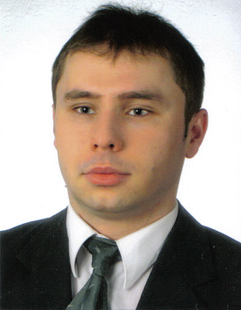
\includegraphics[scale=1.0]{me.jpg}
        \end{textblock}
	\begin{tabular}{rl}
		\textsc{Nazwisko i Imię:} & Ospara Robert \\
		\textsc{Adres:} & ul. Przemyska 24C/8, 80-180 Gdańsk \\
		\textsc{Telefon:} & +48783010280 \\
		\textsc{email:} & \href{mailto:robertospara@gmail.com}{robertospara@gmail.com}
	\end{tabular}
		
    \section{Doświadczenie zawodowe}
        \begin{tabular}{r|p{11cm}}
			\textsc{06.2012-Aktualnie}
			&\emph{Programista/Konsultant}\\
			&\textsc{DC S.A.} (IT)\\
			&\footnotesize{ 
				Odpowiedzialności: tworzenie, rozwijanie i wdrożanie rozwiązań SharePoint-owych. \newline
				Zrealizowane projekty:
				\begin{itemize}
					\item Reporting Status Checker
					\item Pages Generator
					\item Electronic Card Of New Product
					\item TimeSheet.
				\end{itemize}
				Użyte technologie: SharePoint 2010 API, C\#, .NET. Użyte narzędzia: Windows Server 2008 R2, MSSQL, Visual Studio, 
				SVN, Redmine, powershell, LogViewer, SharePoint Designer, MS SQL Management Studio, MS SQL Profiler.
			}\\
			\multicolumn{2}{c}{}\\
	
			\textsc{07.2011-04.2012}
			&\emph{Software Development Engineer}\\
			&\textsc{Samsung Electronics Polska sp. z o.o.} (DTV)\\
			&\footnotesize{ 
				Odpowiedzialności: tworzenie oprogramowania dla platformy telewizji cyfrowej, pisanie narzędzi i testów automatycznych. \newline
				Zrealizowane projekty:
				\begin{itemize}
					\item Software Upgrade (Search Module)
					\item Carousel Dumper
					\item Perforce Efficiency Analyzer.
				\end{itemize}
				Użyte technologie: C++, C, JavaScript, Perl, STL, boost. Użyte narzędzia: Linux, Windows XP, Visual Studio, GNU tools, multiplexers, 
				stream-players, stream-analyzers, stream-converters, Perforce, Jira.
			}\\				
			\multicolumn{2}{c}{}\\
	
			 \textsc{06.2010-04.2011}
			 &\emph{Software Development Engineer} \\
			 &\textsc{Thomson Reuters (Markets) Europe SA Polska} \\
			 & (finanse i bankowość) \\
			 &\footnotesize{
							Odpowiedzialności: Opieka i utrzymanie systemu Kondor+. Używane technologie: C++, SQL(Sybase), STL, boost.
							Używane narzędzia: Solaris, WinXP, Eclipse, shell, AquaStudio, dbxtool, SunStudio, Lotus, 
							SVN.}\\
			 \multicolumn{2}{c}{} \\

			 \textsc{11.2008-02.2009}
			 &\emph{C++ Developer} \\
			 &\textsc{Fluid Desk Sp. Z O.O.} \\
			 & (inżynieria sanitarna) \\
			 &\footnotesize{Dodawanie nowej funkcjonalności do Edytora Bibliotek. Tworzenie dokumentacji technicznej i dla użytkownika. 
							Używane technologie: WinXP, Visual C++, XML, WinAPI, STL, MFC, frameworks. Używane narzędzia: Visual Studio, 
							DOXYGEN, SVN.} \\
			 \multicolumn{2}{c}{} \\

			 \textsc{2004-2008}
			 &\emph{pisanie programów na zamówienie} \\
			 &\footnotesize{Tworzenie aplikacji klient-serwer, stron WWW, aplikacji desktopowych. Używane technologie: WinXP, Linux, 
							Object Pascal, C, C++, Perl, XML, XHTML. Używane narzędzia: Delphi, Anjuta, Geany, shell, scripts, make, 
							gcc, gdb, vim.}\\
			 \multicolumn{2}{c}{} \\

			 \textsc{2002-2006}
			 &\emph{Korepetytor Matematyki, Fizyki i Informatyki} \\
			 &\footnotesize{Nauczanie teorii oraz rozwiązywanie zadań praktycznych w zakresie matematyki, fizyki i informatyki.} \\
			 \multicolumn{2}{c}{} \\

    \end{tabular}

\section{Wykształcenie}
\begin{tabular}{rl}	
	\textsc{10.2000-06.2003}
		& Magister Informatyki \\
	\textsc{10.2006-11.2009}
		& \textbf{Uniwersytet Mikołaja Kopernika w Toruniu} \\
		& \textbf{Wydział Matematyki i Informatyki} \\
		& \textbf{Kierunek Informatyka} \\
		& wykształcenie wyższe \\

	\textsc{09.1996-06.2000}
		& Wykształcenie Średnie - Ogólne - Profilowane \\
		& \textbf{Zespół Szkół Ogólnokształcących} \\
		& \textbf{im. Mikołaja Kopernika w Kołobrzegu} \\
		& \textbf{Profil Specjalności Matematyczno-Fizyczny} \\
		& wykształcenie średnie \\
\end{tabular}
	
    
\section{Odbyte Praktyki}
\begin{tabular}{r|p{11cm}}
	\textsc{07.2005}
	&\emph{Administrator Sieci Komputerowej} \\
	&\textsc{Wojewódzki Szpital Zespolony im. Ludwika Rydygiera w Toruniu} \\
	&\footnotesize{
		Odpowiedzialności: rozwiązywanie problemów ze szpitalną siecią, komputerami i systemami. 
	}\\
	\multicolumn{2}{c}{} \\
		 			
	\textsc{06.2009-08.2009}
	&\emph{Java, C++ Developer} \\
	&\textsc{Tieto Polska sp. z o.o.} \\
	&(telekomunikacja) \\
	&\footnotesize{
		Dodawanie funkcjonalności do produktów rozwijanych przez firmę. Tworzenie aplikacji klient-serwer. Używane 
		technologie: C++, Java, STL, WinAPI. Używane narzędzia: WinXP, MAVEN, Eclipse, Visual Studio.
	}\\
	\multicolumn{2}{c}{} \\
\end{tabular}

\section{Prace Społeczne}
\begin{tabular}{r|p{11cm}}

	\textsc{02.2011-06.2011}
	&\emph{Wolontariusz} \\
	&\textsc{organizacji pożytku publicznego WIOSNA - AFADEMIA PRZYSZŁOŚCI - region trójmiasto} \\
	&\footnotesize{
		Pomoc dzieciom wychowującym się w trudnych warunkach uwierzyć we własne siły i możliwości, 
		w to, że one też są zdolne odnieść SUKCES.
	} \\
	\multicolumn{2}{c}{} \\

	\textsc{2006-2008}
	&\emph{Wolontariusz} \\
	&\textsc{Dom Dziecka Zielony Las w Toruniu} \\
	&\footnotesize{Odrabianie lekcji z dziećmi.} \\
	\multicolumn{2}{c}{} \
\end{tabular}
	
\section{Języki obce}
\begin{tabular}{rl}
	\textsc{angielski:}&bardzo dobrze\\
	\textsc{niemiecki:}&podstawy\\
\end{tabular}

\section{Umiejętności i kompetencje techniczne}
\begin{tabular}{rl}
	\textsc{Języki Programowania}
	&\footnotesize{C++, C\#, C, Perl, JavaScript, Java, Object Pascal} \\
    \multicolumn{2}{c}{} \\
        
    \textsc{Systemy Operacyjne}
    &\footnotesize{Unix, Linux, Windows, Solaris} \\
    \multicolumn{2}{c}{} \\

    \textsc{Inżynieria Oprogramowania}
    &\footnotesize{projektowanie aplikacji, znajomość wzorców architektonicznych i projektowych} \\
    \multicolumn{2}{c}{} \\        
\end{tabular}
	
\section{Informacje dodatkowe}
	Moje hobby to gra na gitarze, gra w szachy, czytanie książek i nauka, a w szczególności fizyka cząstek elementarnych. Interesuję 
	się również: informatyką, nowymi technologiami, astronomią, matematyką, biologią, mikroelektroniką, teologią, muzyką, filmem, 
	rysunkiem i sztukami walki. Reprezentowałem klub Sztorm Kołobrzeg w biegach sprinterskich, a także I LO w Kołobrzegu w Wojewódzkiej 
	Olimpiadzie Młodzieży w koszykówce, na których nasza drużyna zdobyła brązowy medal.
        
    \vfill{}

    \begin{center}
    {\scriptsize Wyrażam zgodę na przetwarzanie danych osobowych, dla potrzeb niezbędnych do realizacji procesu rekrutacji (zgodnie z 
    przepisami ustawy z dn. 29.08.1997r. o ochronie danych osobowych - Dz.U. z 2002 r. nr 101, poz. 926 z póź. zm).}
    \end{center}
	
\end{document}
